\chapter{Evaluation} \label{evaluation}

\section{Overview}
This chapter evaluates the photorealistic scene reconstruction pipeline. The pipeline is divided into two primary stages: post-processing keyframe images and generating a Gaussian splat model. For testing the post-processing script, I created a scene with challenging conditions, including high angular speeds and overexposure, to evaluate the script's ability to filter out unsuitable images. A separate scene with an old microscope was used to test the Gaussian splatting and assess the 3D reconstruction quality. 

\section{Post-Processing Script}
To assess the effectiveness of the post-processing script, I created a dataset with simulated challenging conditions by making rapid movements and positioning a flashlight near the camera. These actions mimicked high angular speeds and overexposure, aiming to introduce blurry and overexposed frames into the dataset. Figure~\ref{fig:keyframes_before_process} shows the saved keyframe images before running the script.

\FloatBarrier
\begin{figure}[htbp]
	\centering
	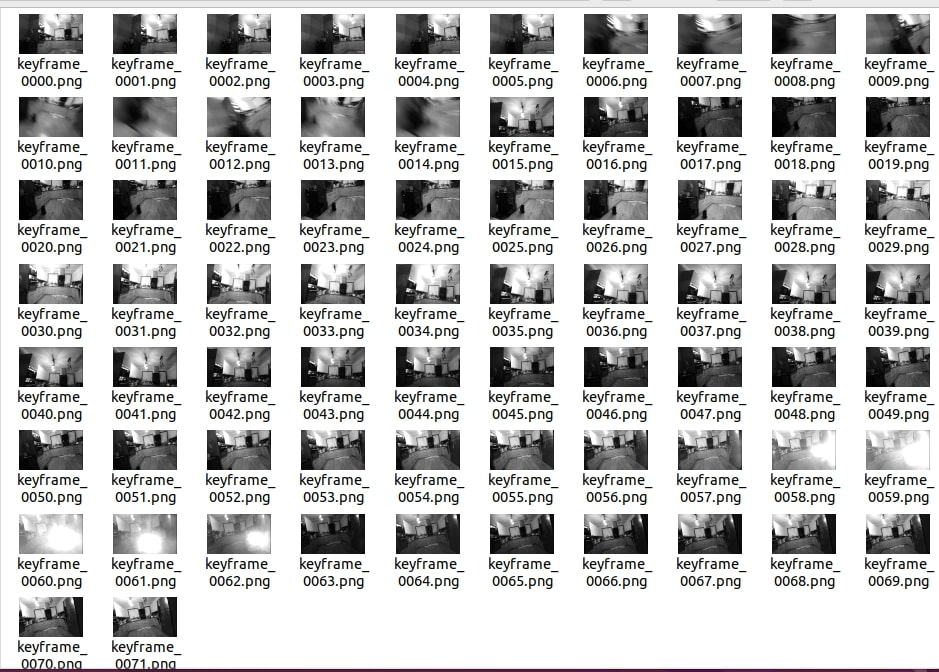
\includegraphics[width=150mm, keepaspectratio]{figures/keyframes_before_process.png}
	\caption{Saved images from mapping by the \textit{keyframe\_saver} node before processing}
	\label{fig:keyframes_before_process}
\end{figure}
\FloatBarrier

After running the script, which detected and removed blurry or overexposed frames, the processed image set can be seen in Figure~\ref{fig:keyframes_after_process}. The script’s output, detailing deletions and renamings, is shown in Figure~\ref{fig:image_process_script_output}. Examples of detected blurry and overexposed images that the script correctly flagged for deletion are displayed in Figure~\ref{fig:blurry_overexposed_example}.

\FloatBarrier
\begin{figure}[htbp]
	\centering
	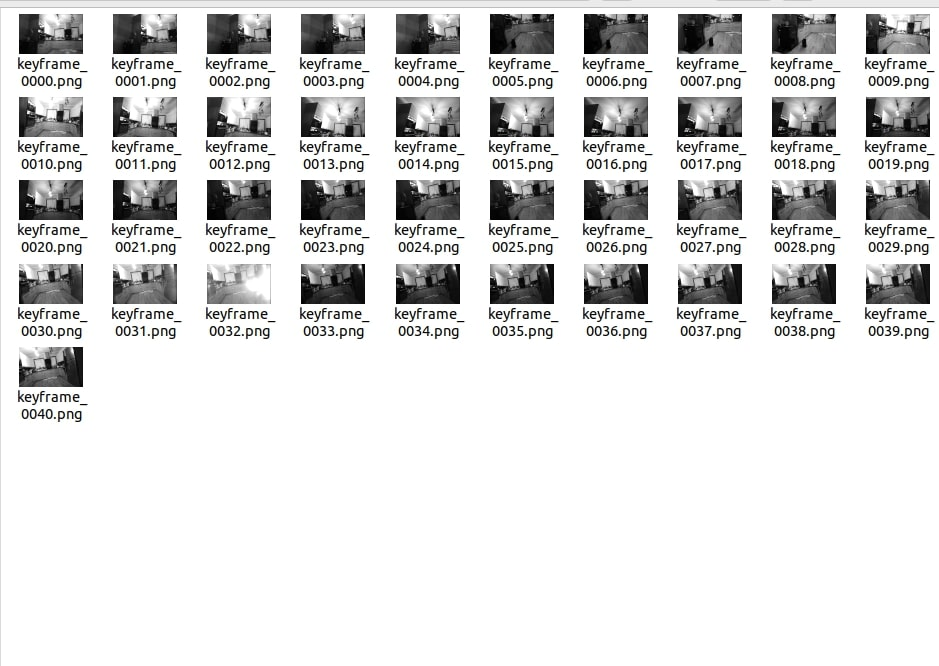
\includegraphics[width=150mm, keepaspectratio]{figures/keyframes_after_process.png}
	\caption{Remaining images after running the post-processing script}
	\label{fig:keyframes_after_process}
\end{figure}

\begin{figure}[htbp]
	\centering
	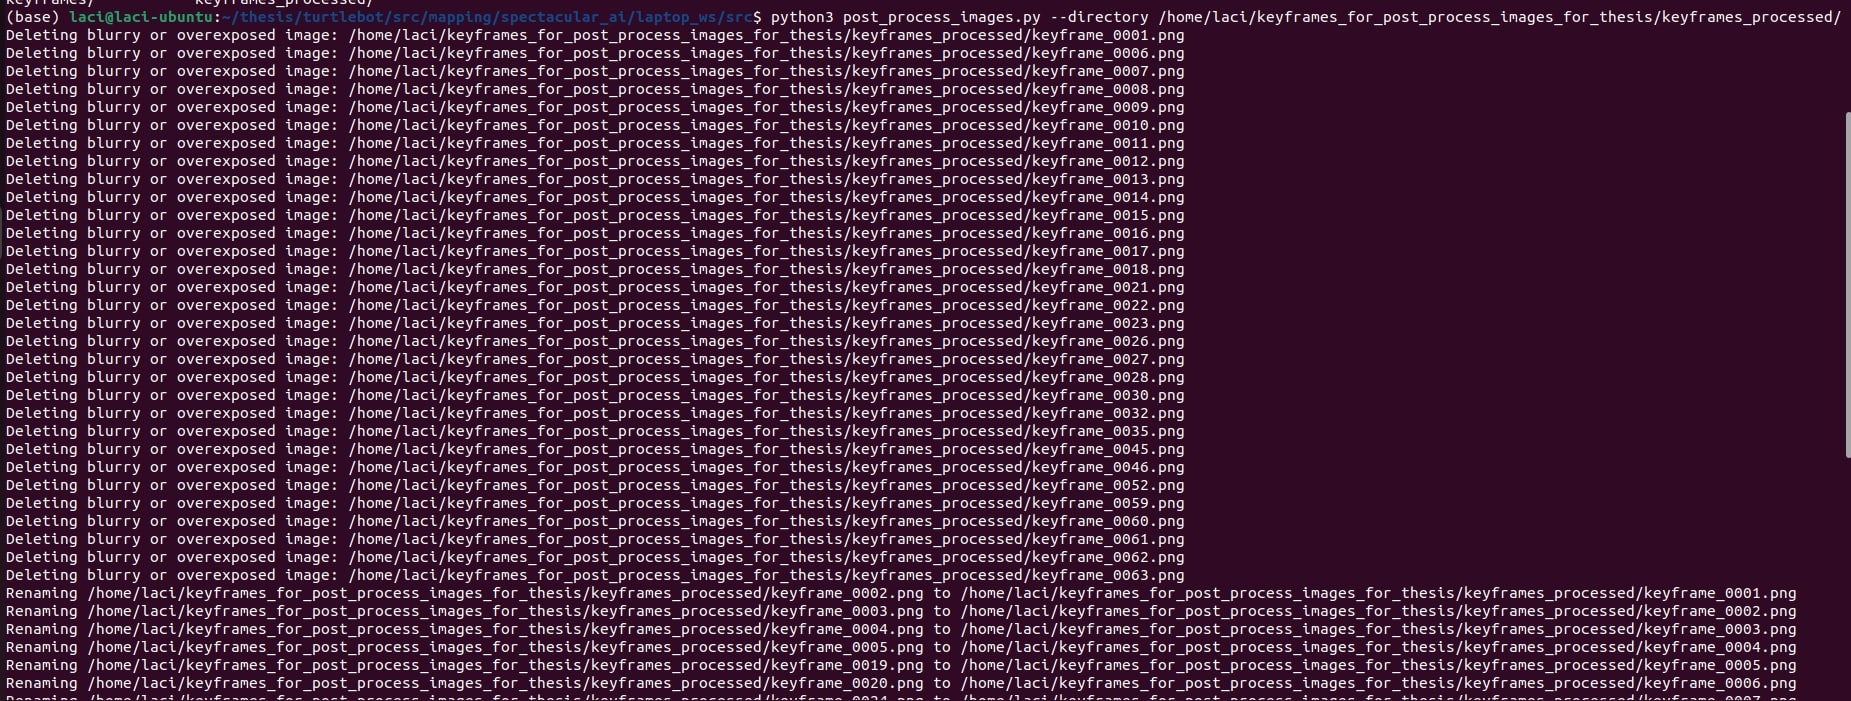
\includegraphics[width=150mm, keepaspectratio]{figures/process_script_output.png}
	\caption{Terminal output of the post-processing script}
	\label{fig:image_process_script_output}
\end{figure}


\begin{figure}[htbp]
	\centering
	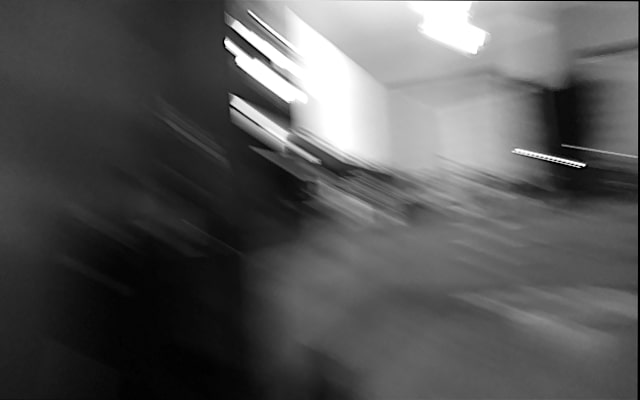
\includegraphics[width=67mm, keepaspectratio]{figures/example_for_blurry.png}\hspace{1cm}
	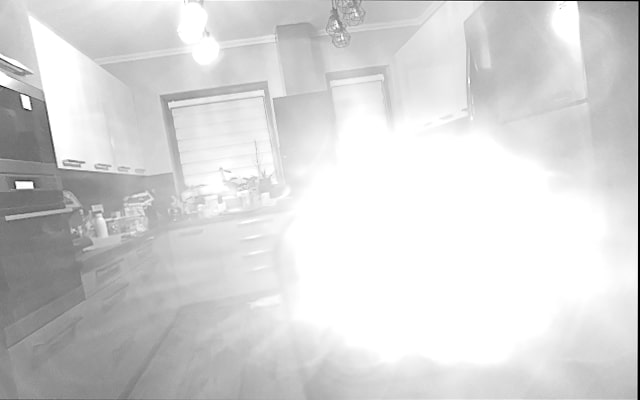
\includegraphics[width=67mm, keepaspectratio]{figures/example_for_overexposed.png}\\\vspace{5mm}
	\caption{Examples of blurry (left) and overexposed (right) images successfully detected and deleted by the script}
	\label{fig:blurry_overexposed_example}
\end{figure}
\FloatBarrier

\section{Gaussian Splatting}
To evaluate the Gaussian splatting capabilities, I recorded a scene with an old microscope, positioned centrally in a controlled setting. After running the post-processing script to filter the images, I trained the \verb|splatfacto-big| model on the processed dataset. Figure~\ref{fig:spai_gsplat} displays the reconstructed splat.

\begin{figure}[htbp]
	\centering
	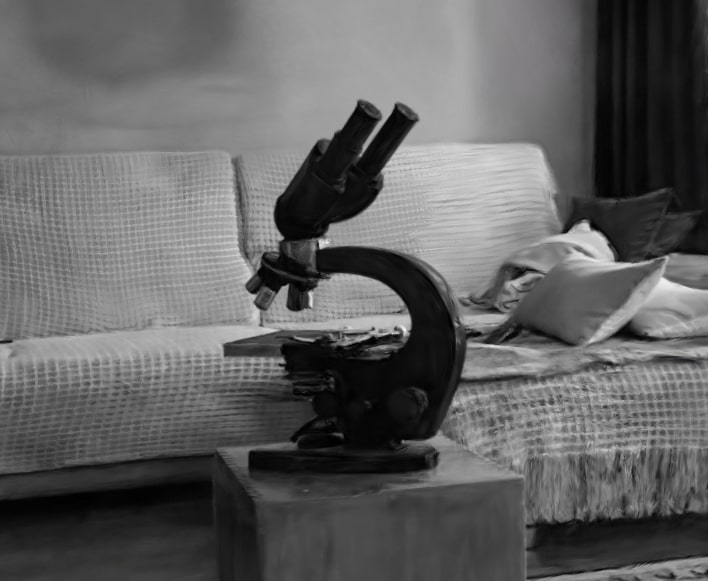
\includegraphics[width=150mm, keepaspectratio]{figures/spai_gsplat.png}
	\caption{Reconstructed microscope scene using Gaussian splatting}
	\label{fig:spai_gsplat}
\end{figure}

The reconstructed item appears slightly blurry, with some dark areas within the image. This effect results from the high amount of incoming light through windows positioned to the right of the capture area, which introduces lighting variations and subtle perturbations to the Gaussian splatting process. Additionally, the generated splat is in grayscale, as the mapping node uses the Spectacular AI Python SDK's camera pipeline. This SDK exclusively utilizes grayscale stereo cameras, omitting the RGB camera. Unfortunately, the pipeline configuration is fixed, so activating the RGB camera was not an option. However, given the spatial calculation speed and accuracy provided by this SDK, we chose to prioritize these qualities over color data. Implementing a custom spatial camera pipeline to support RGB capture was evaluated but ultimately deemed too time-intensive for our timeline.

Overall, this pipeline enables high-quality, photorealistic reconstructions, even without RGB data. Despite the grayscale limitation, the combination of Gaussian splatting and the Spectacular AI SDK’s stereo-based spatial accuracy produces detailed and realistic 3D models. The pipeline captures fine spatial features and preserves depth and texture fidelity, creating a solid foundation for effective reconstructions in real-world settings.



TODO: write more about these images

\begin{figure}[htbp]
	\centering
	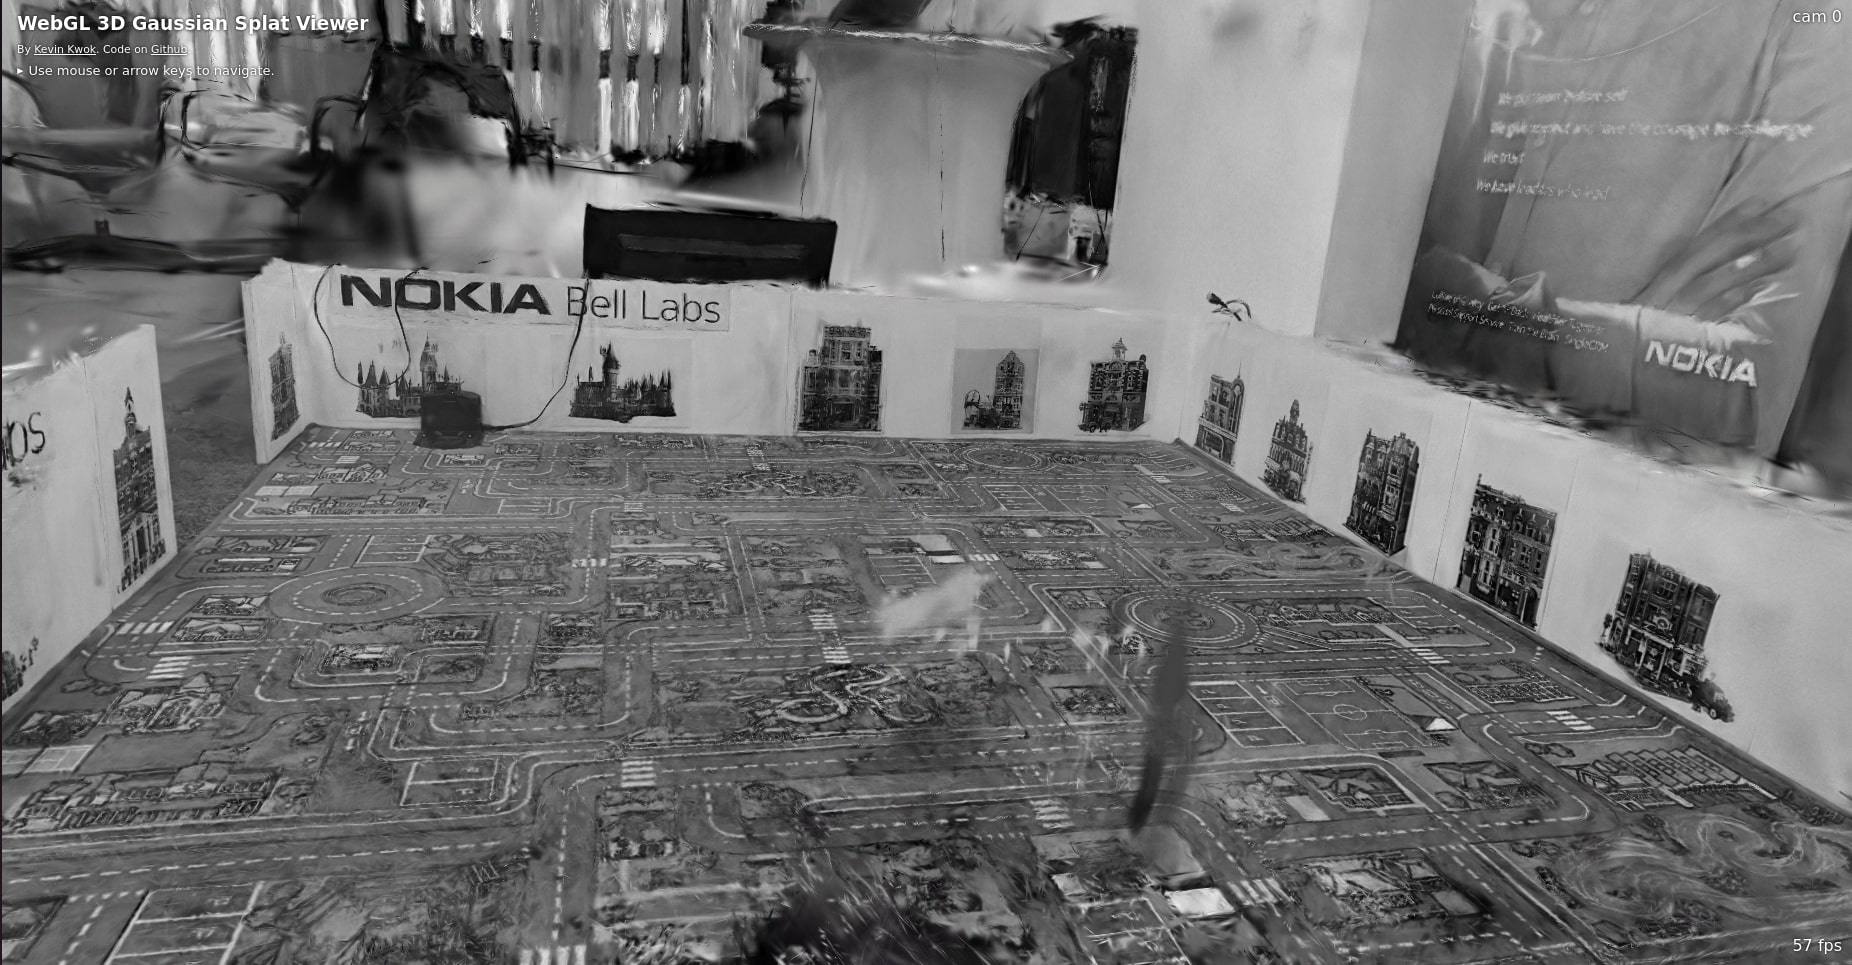
\includegraphics[width=150mm, keepaspectratio]{figures/nokia_splat_splatfacto_big_1.png}
	\caption{Reconstructed map in the Nokia office with the \tectit{splatfacto-big} model}
	\label{fig:nokia_splatfacto_big_1}
\end{figure}


\begin{figure}[htbp]
	\centering
	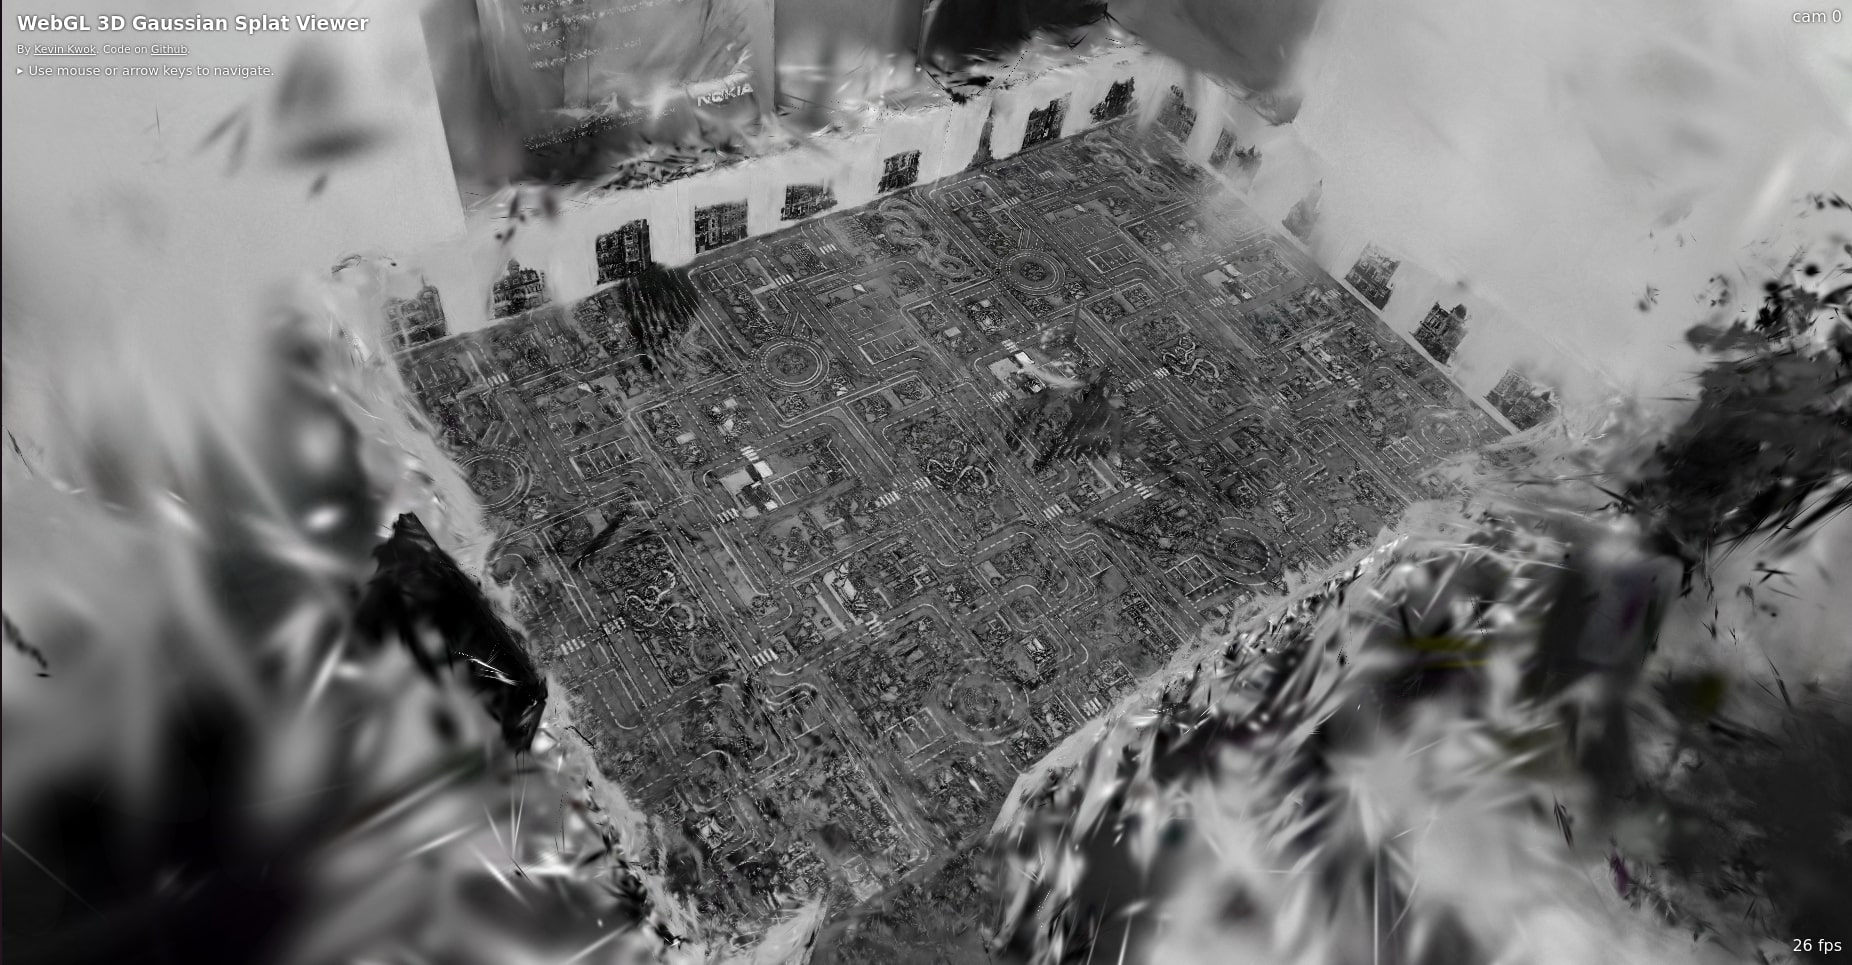
\includegraphics[width=150mm, keepaspectratio]{figures/nokia_splat_splatfacto_big_2.png}
	\caption{Reconstructed map in the Nokia office with the \tectit{splatfacto-big} model}
	\label{fig:nokia_splatfacto_big_2}
\end{figure}


\begin{figure}[htbp]
	\centering
	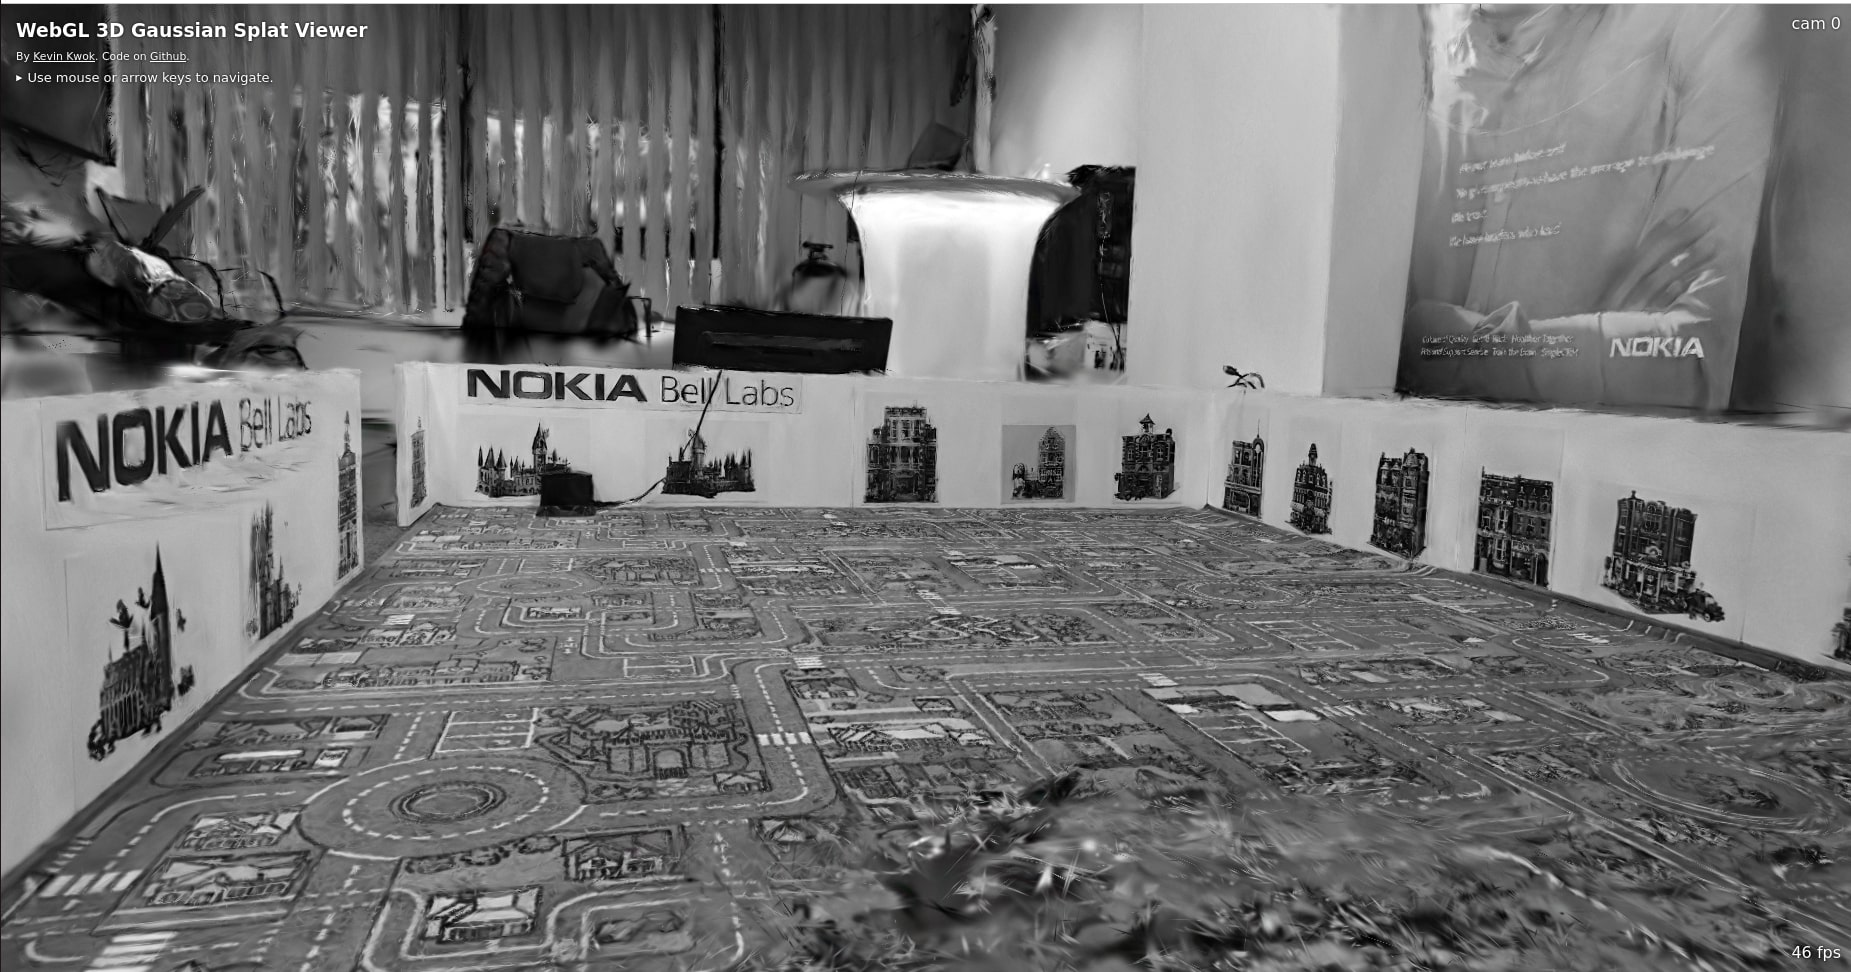
\includegraphics[width=150mm, keepaspectratio]{figures/nokia_splatfacto_1.png}
	\caption{Reconstructed map in the Nokia office with the \textit{splatfacto} model}
	\label{fig:nokia_splatfacto_1}
\end{figure}

\begin{figure}[htbp]
	\centering
	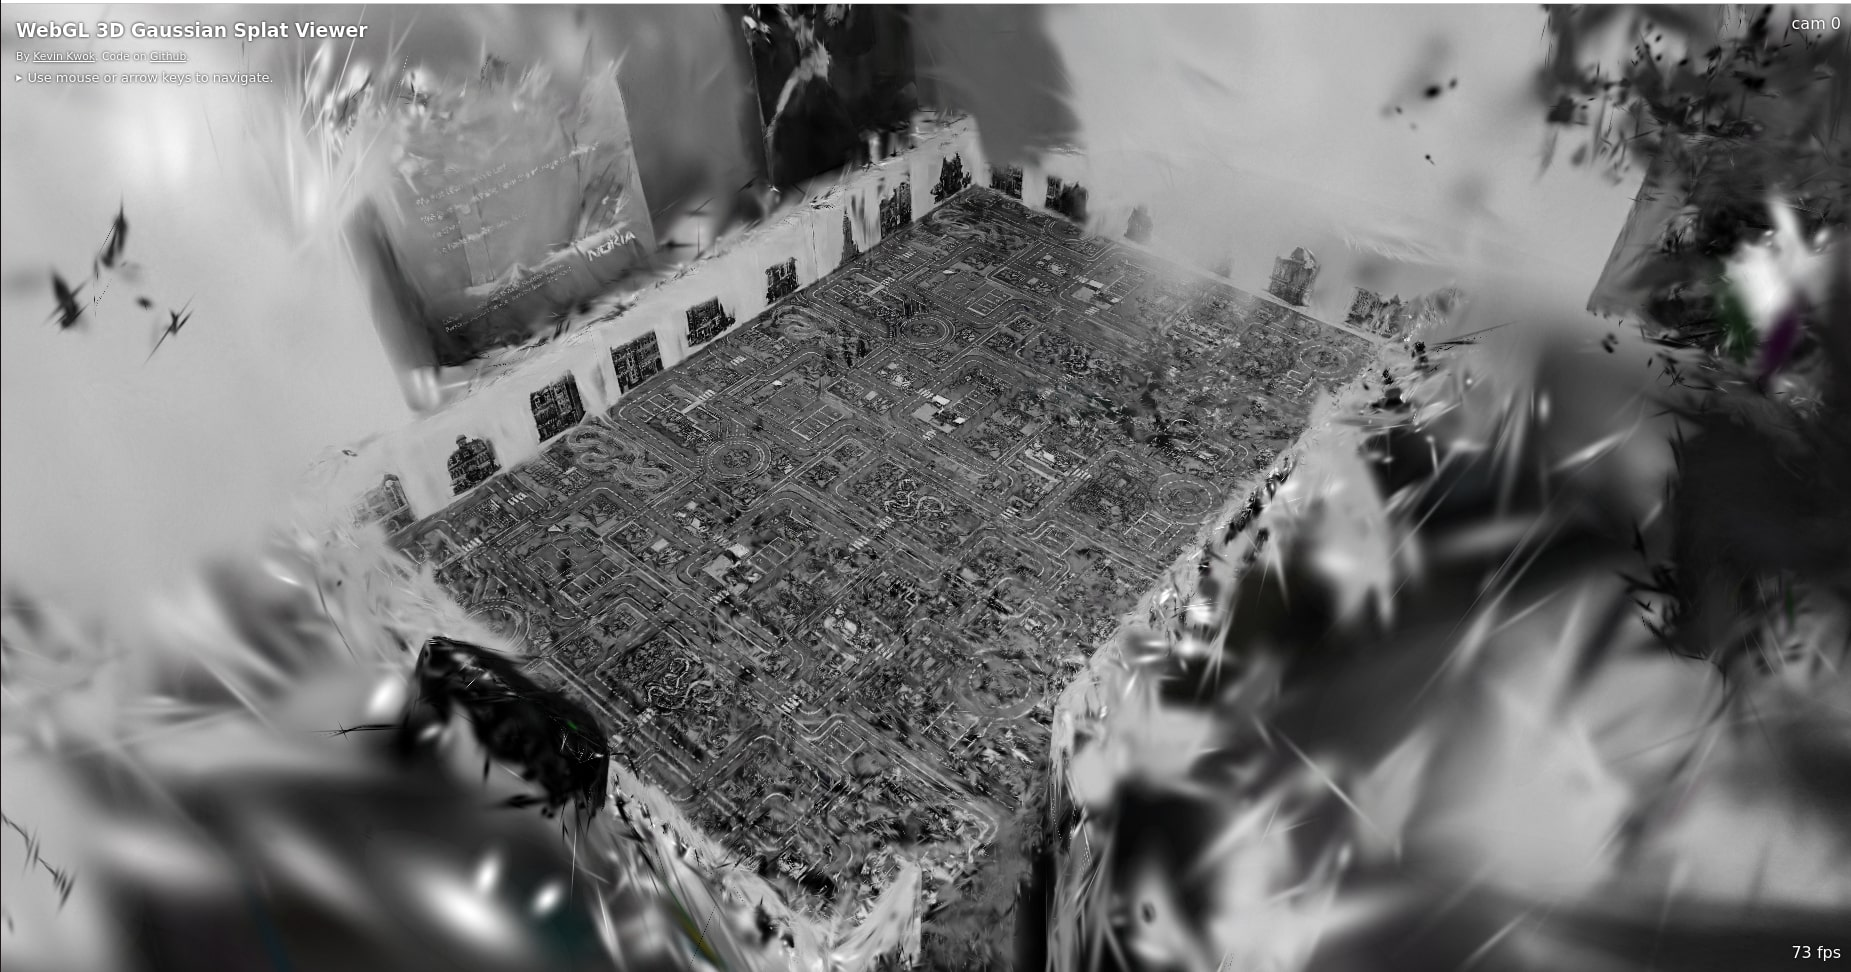
\includegraphics[width=150mm, keepaspectratio]{figures/nokia_splatfacto_2.png}
	\caption{Reconstructed map in the Nokia office with the \tectit{splatfacto} model}
	\label{fig:nokia_splatfacto_2}
\end{figure}

